\documentclass[11pt]{beamer}
%\documentclass[11pt, aspectratio=169]{beamer}
\usepackage[utf8]{inputenc}
\usepackage[ngerman]{babel}
\usepackage{tikz}
\usetikzlibrary{shadows}
\usepackage{graphicx}
\usepackage[many]{tcolorbox}

\usetheme{TuDo}
\begin{document}
	\author{Michael R. und Timon S.}
	\title{Smart Mirror}
	\subtitle{Proseminar}
	\institute{TU Dortmund - Fakult\"at f\"ur Informatik}
	\date{\today}
	%\subject{}
	%\setbeamercovered{transparent}
	\titlegraphic{
		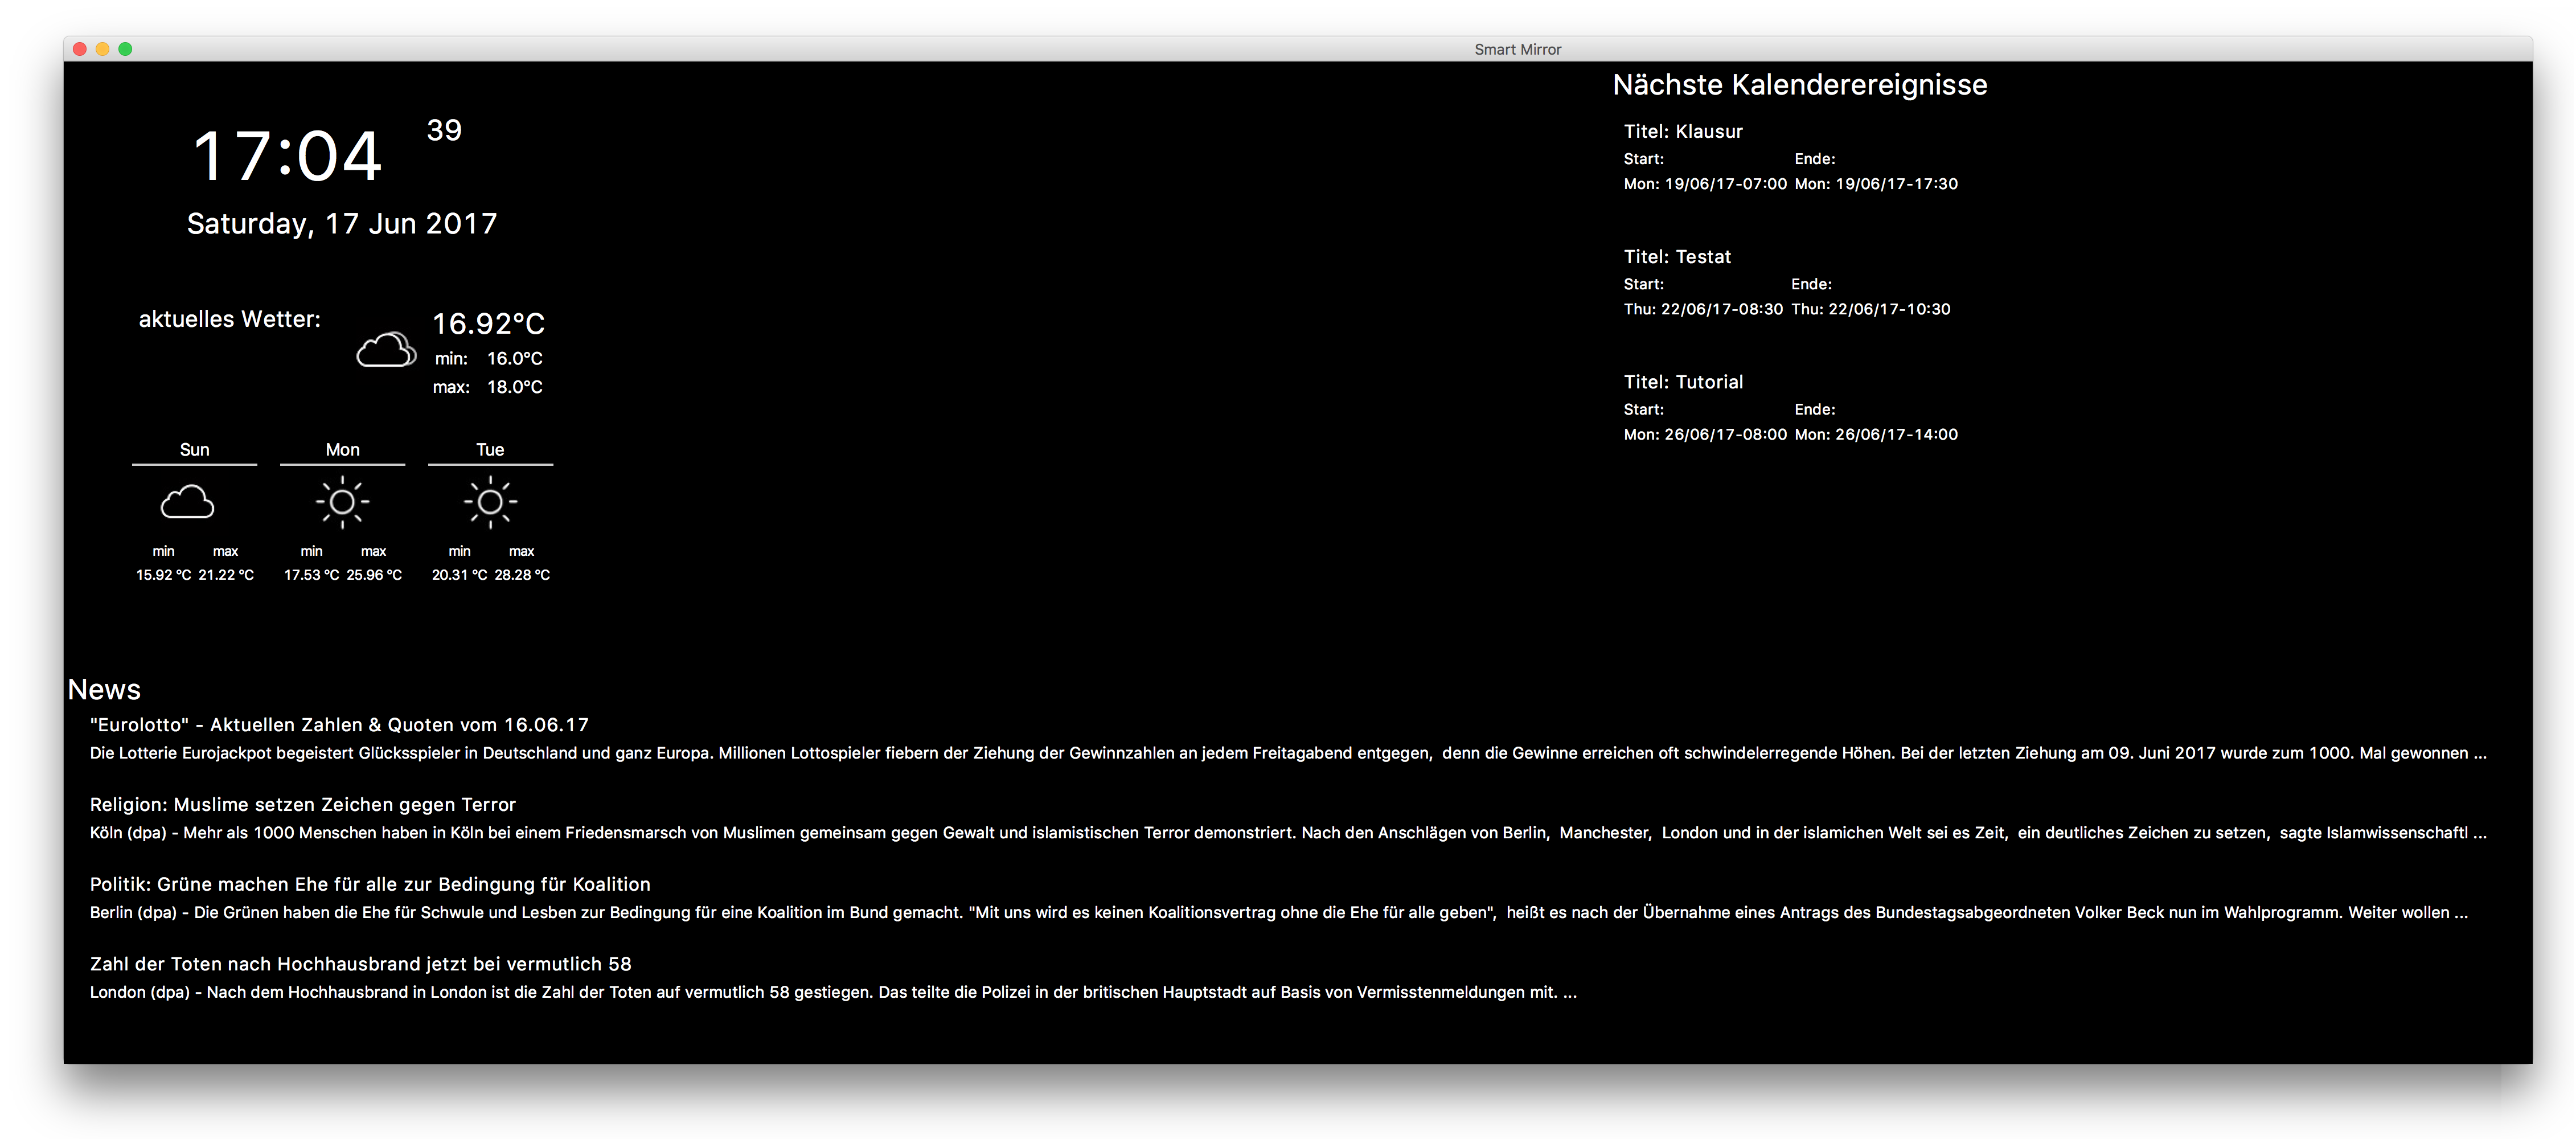
\includegraphics[width=0.35\paperwidth]{images/titlepage}
	}
	
	\begin{frame}
		\titlepage
	\end{frame}

	\begin{frame}
		\frametitle{Frage}
		\centering
		\huge
		\vfill
		Vergisst du auch h\"aufig den Geburtstag deiner Großeltern?
		\vfill
	\end{frame}

	\begin{frame}
		\frametitle{L\"osung}
		\centering
		\Large
		So kann dir das nicht mehr passieren!
		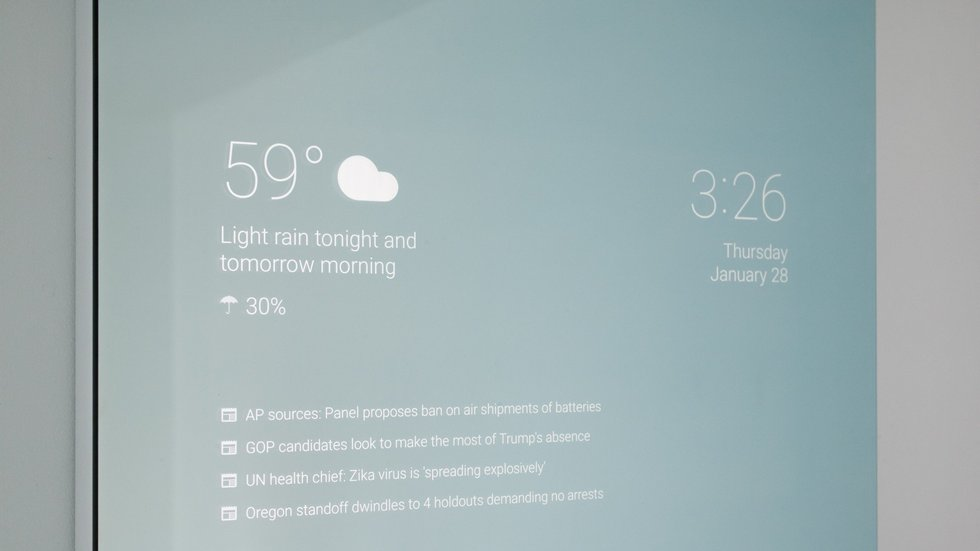
\includegraphics[width = .7\paperwidth]{images/showcaseImage}
	\end{frame}

	\begin{frame}
		\frametitle{Übersicht}
		\tableofcontents
	\end{frame}

	\section{Verteilung der Aufgaben}
	\begin{frame}
		\frametitle{Verteilung der Aufgaben}
	\end{frame}

	\section{technische Komponenten}
	\begin{frame}
		\frametitle{Hardwaregruppen}
		\begin{center}
			\Large{Aufteilung in Bereiche}
		\end{center}
		\begin{itemize}
		\item Ikearahmen 50x50 cm
		\item Displayeinheit
		\item Raspberry Pi und Sensoren
		\item Stromversorgung
		\end{itemize}
	\end{frame}
	
	\begin{frame}
		\frametitle{Rahmenaufbau}
	\end{frame}		

	\begin{frame}
		\frametitle{Technische Komponenten}
		\begin{itemize}
		\item 17 Zoll Monitor Format 4:3
		\item Netzteil für Monitor
		\item Display Controller HDMI zu IPEX-40Pin LVDS Kabel 
		\item Raspberry Pi 3
		\item Bewegungsmelder
		\item Temepraturfühler
		\item 5V Netzteil
		\item HDMI zu VGA Adapter
		\end{itemize}
	\end{frame}

	\subsection{Explosionsskizze}
	\begin{frame}
		\frametitle{Verteilungsdiagramm}
		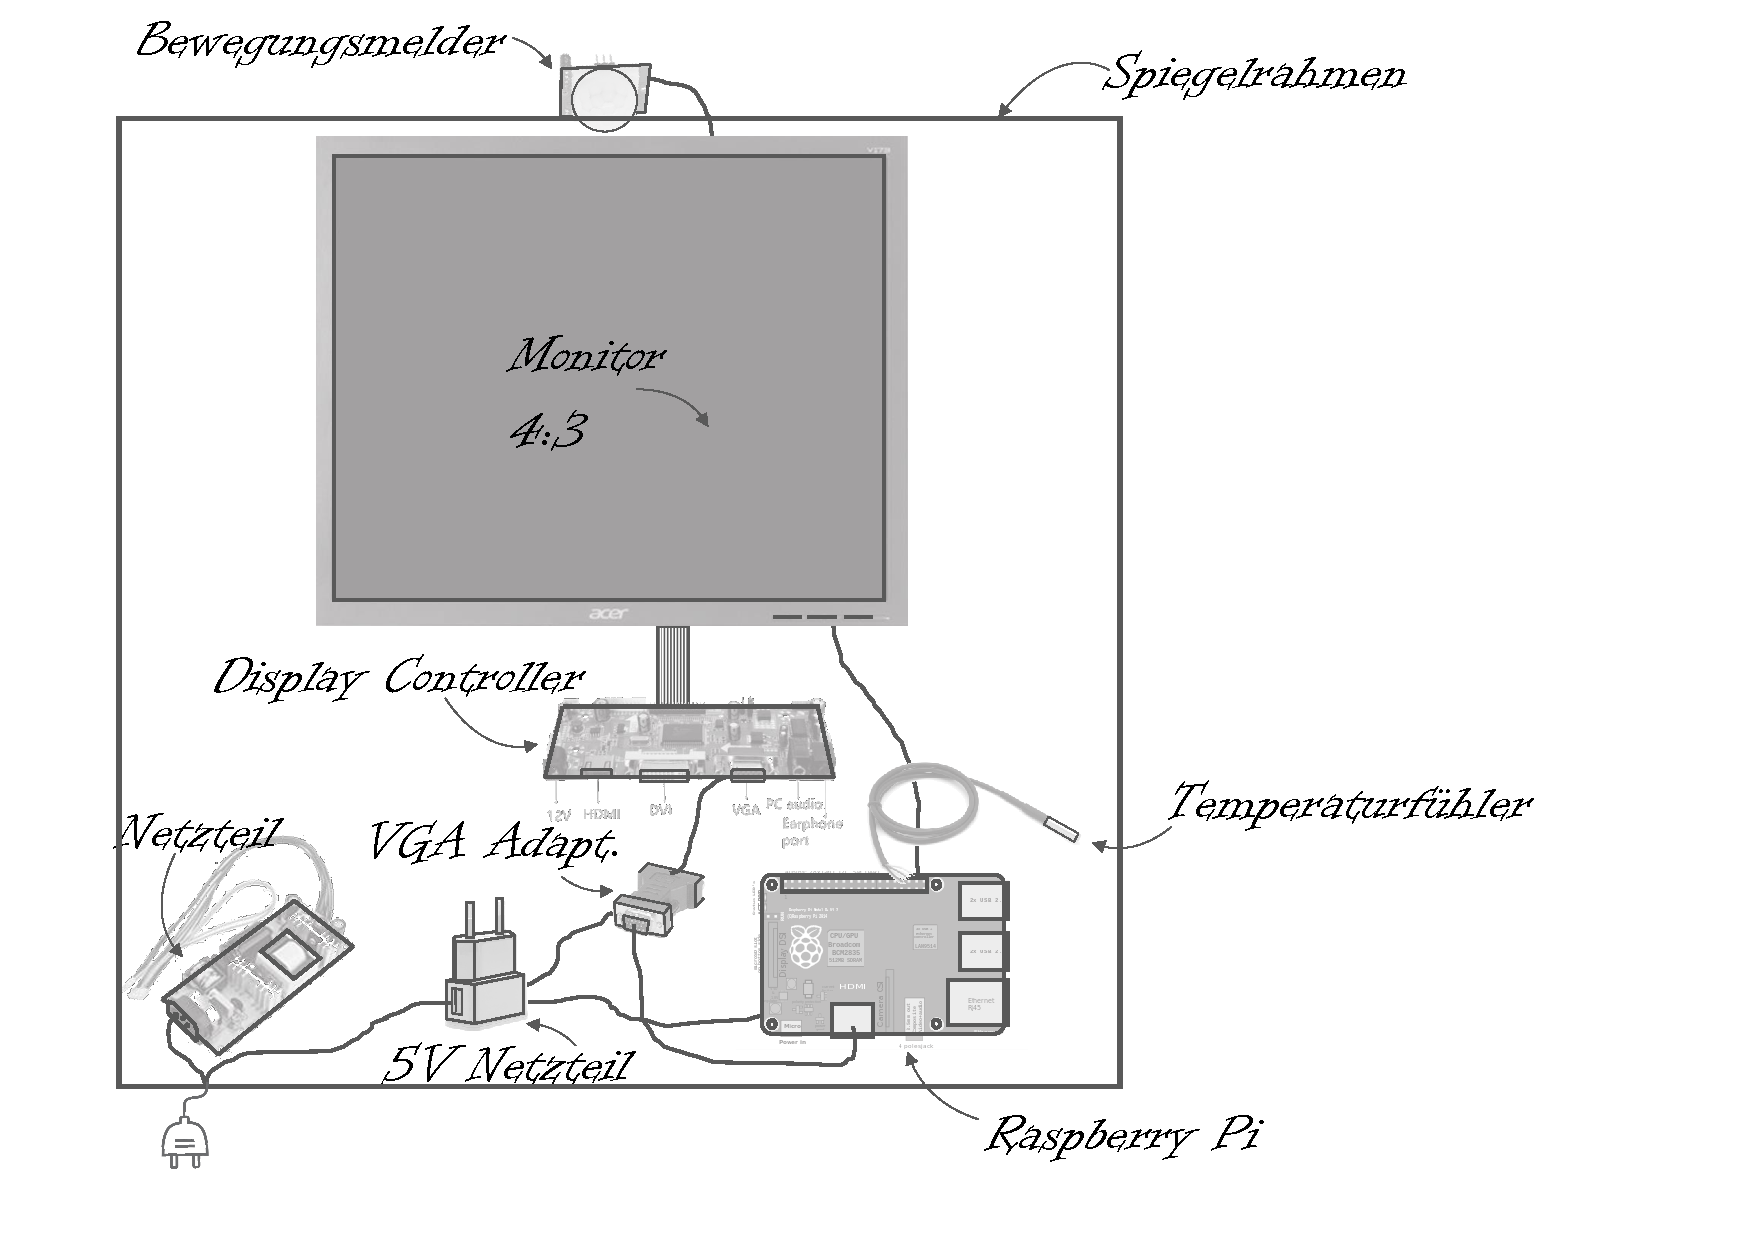
\includegraphics[scale = 0.4]{images/smartMirrorExplosionsskizze.pdf}
	\end{frame}

	\section{UI}
	\begin{frame}
		\frametitle{Graphische Oberfl\"ache}
		\begin{center}
			
\includegraphics[scale=0.3]{images/python+tkinter.png}
			\linebreak
			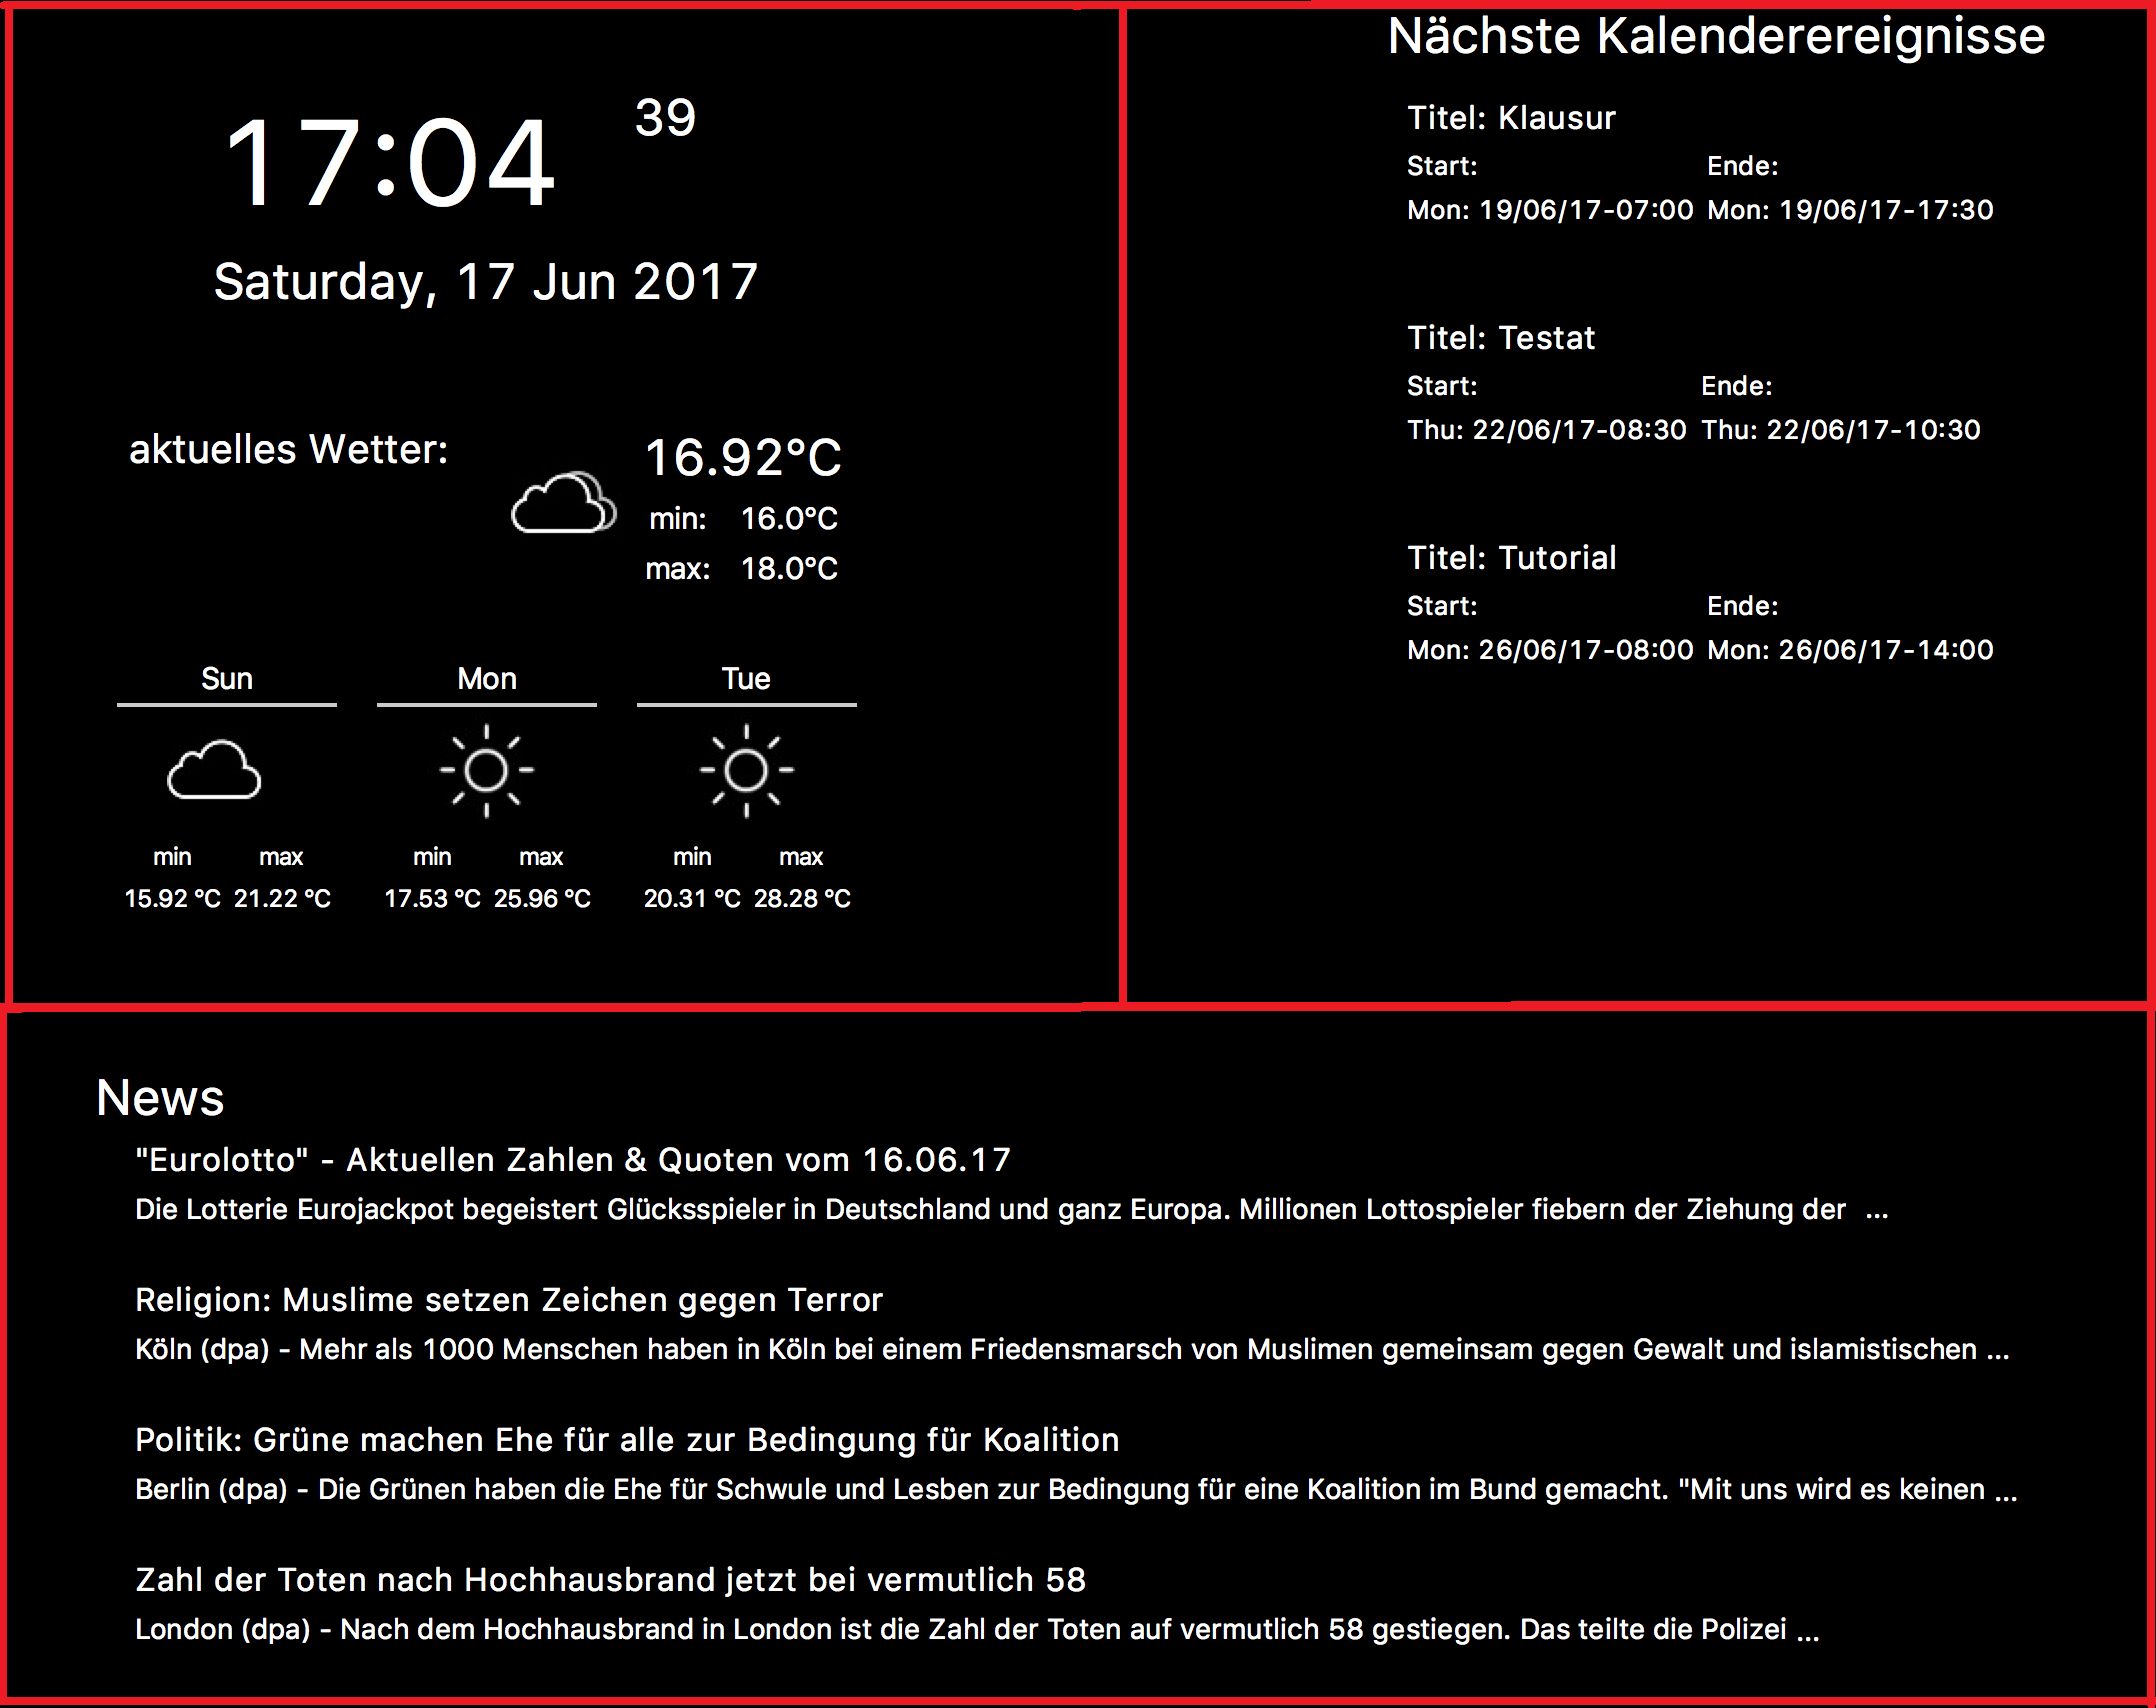
\includegraphics[scale=0.2]{images/grafOberflaeche.png}
		\end{center}
	\end{frame}
		
	\section{Programmierung}
	\subsection{Integration des MVC-Patterns}
	\begin{frame}
		\frametitle{Projektstruktur}
	\end{frame}

	\subsection{genutzte API's}
	\begin{frame}
		\frametitle{genutzte API's}
	\end{frame}

	
	\section{Fazit}
	\begin{frame}
		\frametitle{Fazit}
	\end{frame}
\end{document}